\documentclass[11pt,a4paper]{article}

% ============================================================
% PACKAGES
% ============================================================
\usepackage[margin=1in]{geometry}
\usepackage{titlesec}
\usepackage{enumitem}
\usepackage{graphicx}
\usepackage{tikz}
\usetikzlibrary{shapes,arrows,positioning,calc}
\usepackage{pgfgantt}
\usepackage{hyperref}
\usepackage{xcolor}
\usepackage{amsmath}
\usepackage{booktabs}
\usepackage{listings}
\usepackage{fancyhdr}
\usepackage{caption}
\usepackage{subcaption}

% ============================================================
% COLORS
% ============================================================
\definecolor{primarycolor}{RGB}{0,102,204}
\definecolor{secondarycolor}{RGB}{204,0,0}
\definecolor{codegreen}{RGB}{0,128,0}
\definecolor{codegray}{RGB}{128,128,128}
\definecolor{codepurple}{RGB}{128,0,128}
\definecolor{backcolour}{RGB}{245,245,245}

% ============================================================
% HYPERREF SETUP
% ============================================================
\hypersetup{
    colorlinks=true,
    linkcolor=primarycolor,
    filecolor=magenta,      
    urlcolor=primarycolor,
    citecolor=primarycolor,
    pdftitle={Prompt Crash-Test Lab: LLM Robustness Benchmark},
    pdfauthor={Your Name},
}

% ============================================================
% CODE LISTING SETUP
% ============================================================
\lstdefinestyle{mystyle}{
    backgroundcolor=\color{backcolour},   
    commentstyle=\color{codegreen},
    keywordstyle=\color{blue},
    numberstyle=\tiny\color{codegray},
    stringstyle=\color{codepurple},
    basicstyle=\ttfamily\footnotesize,
    breakatwhitespace=false,         
    breaklines=true,                 
    captionpos=b,                    
    keepspaces=true,                 
    numbers=left,                    
    numbersep=5pt,                  
    showspaces=false,                
    showstringspaces=false,
    showtabs=false,                  
    tabsize=2
}
\lstset{style=mystyle}

% ============================================================
% TITLE FORMATTING
% ============================================================
\titleformat{\section}
  {\normalfont\Large\bfseries\color{primarycolor}}{\thesection}{1em}{}
\titleformat{\subsection}
  {\normalfont\large\bfseries\color{primarycolor}}{\thesubsection}{1em}{}

% ============================================================
% HEADER/FOOTER
% ============================================================
\pagestyle{fancy}
\fancyhf{}
\fancyhead[L]{\small CS 599 - Contemporary Developments}
\fancyhead[R]{\small Prompt Crash-Test Lab}
\fancyfoot[C]{\thepage}

% ============================================================
% DOCUMENT START
% ============================================================
\begin{document}

% ============================================================
% TITLE PAGE
% ============================================================
\begin{titlepage}
    \centering
    \vspace*{2cm}
    
    {\Huge\bfseries Prompt Crash-Test Lab\par}
    \vspace{0.5cm}
    {\Large\itshape LLM Robustness Benchmark Framework\par}
    \vspace{2cm}
    
    {\Large CS 599: Contemporary Developments\par}
    {\Large (Applications of Large Language Models)\par}
    \vspace{1cm}
    
    {\large\bfseries Project Proposal Document\par}
    \vspace{2cm}
    
    {\Large
    \textbf{Author:} Your Name Here \\
    \texttt{your.email@university.edu} \\
    \vspace{0.5cm}
    \textbf{Partner:} Partner Name (if applicable) \\
    \texttt{partner.email@university.edu}
    \par}
    
    \vfill
    
    {\large February 23, 2026\par}
\end{titlepage}

% ============================================================
% TABLE OF CONTENTS
% ============================================================
\tableofcontents
\newpage

% ============================================================
% PART 1: MAIN PROJECT PROPOSAL (2 PAGES)
% ============================================================
\part{Project Proposal}

\section{Project Overview and Motivation}

\subsection{Background and Problem Statement}

Large Language Models (LLMs) have become integral to modern software systems, powering applications from code generation to customer service. However, a critical challenge persists: \textbf{prompt sensitivity and inconsistent behavior}. Recent studies demonstrate that seemingly equivalent prompt formulations can yield drastically different outputs—variations in phrasing, formatting, or instruction order can cause accuracy fluctuations of 20-40\%.

This inconsistency poses severe risks in production environments:

\begin{itemize}[leftmargin=*]
    \item \textbf{Reliability issues}: Minor prompt changes break deployed systems
    \item \textbf{Security vulnerabilities}: Adversarial users can manipulate outputs through prompt injection
    \item \textbf{Cost unpredictability}: Token usage varies wildly across equivalent prompts
    \item \textbf{Quality assurance challenges}: No systematic method to test prompt robustness before deployment
\end{itemize}

\subsection{Why This Project is Needed}

Currently, developers rely on ad-hoc testing and intuition when crafting prompts. There exists \textbf{no standardized framework} for:

\begin{enumerate}[leftmargin=*]
    \item Automatically generating semantically equivalent prompt variants
    \item Measuring consistency across these variants
    \item Comparing robustness across different LLM providers
    \item Identifying which prompt characteristics cause instability
\end{enumerate}

This project addresses a fundamental gap in LLM deployment practices by creating a reproducible benchmark and testing harness that quantifies prompt robustness.

\subsection{Real-World Impact}

Organizations deploying LLMs face significant financial and reputational risks from prompt instability. A single poorly-tested prompt can:

\begin{itemize}[leftmargin=*]
    \item Generate incorrect structured data (e.g., invalid JSON breaking downstream systems)
    \item Hallucinate facts in customer-facing applications
    \item Exhibit bias or inappropriate content based on minor phrasing differences
    \item Cost thousands in wasted API calls during debugging
\end{itemize}

By providing quantitative robustness metrics, this project enables evidence-based prompt engineering and safer LLM deployment.

\section{Primary Objectives and Goals}

\subsection{Main Objective}

Develop an automated framework that \textbf{systematically evaluates LLM robustness} by generating prompt variants, executing them across multiple models, and producing comprehensive stability metrics.

\subsection{Specific Goals}

\begin{enumerate}[leftmargin=*]
    \item \textbf{Create a reusable benchmark dataset} containing:
    \begin{itemize}
        \item 100+ base prompts across two task categories
        \item 10-30 automatically generated variants per base prompt
        \item Ground truth labels for objective evaluation
    \end{itemize}
    
    \item \textbf{Build an evaluation harness} that:
    \begin{itemize}
        \item Executes prompts across 4+ LLM providers (GPT-4, Claude, Gemini, Llama)
        \item Caches results to minimize API costs
        \item Supports batching and parallel execution
    \end{itemize}
    
    \item \textbf{Implement comprehensive metrics}:
    \begin{itemize}
        \item Semantic consistency (embedding similarity)
        \item Format compliance (schema validation)
        \item Answer correctness (against ground truth)
        \item Stability score (variance across variants)
    \end{itemize}
    
    \item \textbf{Generate actionable insights}:
    \begin{itemize}
        \item Identify which models are most/least robust
        \item Determine which prompt characteristics cause instability
        \item Recommend best practices for prompt design
    \end{itemize}
    
    \item \textbf{Produce publishable research}:
    \begin{itemize}
        \item Reproducible experimental methodology
        \item Statistical analysis of results
        \item Open-source code and datasets
    \end{itemize}
\end{enumerate}

\subsection{Problems Solved}

\begin{itemize}[leftmargin=*]
    \item \textbf{Lack of standardization}: Provides common benchmark for comparing LLM robustness
    \item \textbf{Manual testing burden}: Automates generation and evaluation of prompt variants
    \item \textbf{Opaque failure modes}: Reveals specific conditions under which models become unstable
    \item \textbf{Model selection uncertainty}: Offers empirical data for choosing appropriate LLMs
\end{itemize}

\section{Project Scope}

\subsection{What is Included}

\begin{enumerate}[leftmargin=*]
    \item \textbf{Two Task Categories:}
    \begin{itemize}
        \item \textbf{JSON Extraction}: Structured data extraction with schema validation
        \item \textbf{Grounded Question Answering}: Context-based Q\&A requiring citation
    \end{itemize}
    
    \item \textbf{Prompt Variant Generation:}
    \begin{itemize}
        \item Paraphrasing (semantic equivalence)
        \item Formatting changes (markdown, plaintext, structured)
        \item Role modifications (system prompts, user personas)
        \item Constraint additions (length limits, tone requirements)
        \item Template variations (few-shot examples, chain-of-thought)
    \end{itemize}
    
    \item \textbf{Model Coverage:}
    \begin{itemize}
        \item OpenAI GPT-4-turbo
        \item Anthropic Claude 3.5 Sonnet
        \item Google Gemini 1.5 Pro
        \item Meta Llama 3.1 70B
    \end{itemize}
    
    \item \textbf{Evaluation Metrics:}
    \begin{itemize}
        \item Robustness score (consistency across variants)
        \item Accuracy (correctness vs ground truth)
        \item Format compliance (schema/constraint adherence)
        \item Semantic stability (embedding similarity)
        \item Cost efficiency (tokens per correct answer)
    \end{itemize}
    
    \item \textbf{Deliverables:}
    \begin{itemize}
        \item Benchmark dataset (JSONL format)
        \item Python evaluation framework
        \item Interactive dashboard (Streamlit)
        \item Technical report with findings
        \item Open-source repository
    \end{itemize}
\end{enumerate}

\subsection{What is Excluded}

To maintain feasible scope, the following are \textbf{explicitly excluded}:

\begin{itemize}[leftmargin=*]
    \item \textbf{Multimodal inputs}: Images, audio, video (text-only)
    \item \textbf{Fine-tuning experiments}: Using only pre-trained models via API
    \item \textbf{Production deployment}: Proof-of-concept only, not production-ready
    \item \textbf{Advanced adversarial attacks}: Focus on benign variation, not jailbreaking
    \item \textbf{Real-time evaluation}: Batch processing only
    \item \textbf{Custom model hosting}: API-based models only
    \item \textbf{Non-English languages}: English prompts and responses only
\end{itemize}

\subsection{Boundaries and Limitations}

\begin{itemize}[leftmargin=*]
    \item Dataset size limited to 100-150 base prompts (1500-3000 total variants)
    \item Budget constraint: \$200 maximum for API costs
    \item Timeline: 4 weeks for complete implementation
    \item Team size: 1-2 members
\end{itemize}

\section{Main Tasks and Activities}

\subsection{Phase 1: Dataset Creation (Week 1)}

\begin{enumerate}[leftmargin=*]
    \item \textbf{Task 1.1}: Design JSON extraction schemas
    \begin{itemize}
        \item Define 5 domain schemas (e-commerce, medical, finance, etc.)
        \item Create sample documents and ground truth labels
        \item Validate schema complexity (3-10 fields each)
    \end{itemize}
    
    \item \textbf{Task 1.2}: Develop grounded Q\&A dataset
    \begin{itemize}
        \item Select 50 Wikipedia/documentation paragraphs
        \item Write questions requiring context citation
        \item Label correct answers with supporting quotes
    \end{itemize}
    
    \item \textbf{Task 1.3}: Build variant generator
    \begin{itemize}
        \item Implement paraphrasing using GPT-4
        \item Create formatting templates
        \item Develop role/constraint modifiers
    \end{itemize}
    
    \item \textbf{Task 1.4}: Generate and validate variants
    \begin{itemize}
        \item Produce 10-30 variants per base prompt
        \item Manual review of 10\% sample for quality
        \item Store in structured JSONL format
    \end{itemize}
\end{enumerate}

\subsection{Phase 2: Evaluation Framework (Week 2)}

\begin{enumerate}[leftmargin=*]
    \item \textbf{Task 2.1}: Implement API integration layer
    \begin{itemize}
        \item Create unified interface for 4 model providers
        \item Add retry logic and error handling
        \item Implement response caching (SQLite)
    \end{itemize}
    
    \item \textbf{Task 2.2}: Build batch execution engine
    \begin{itemize}
        \item Parallel processing with rate limiting
        \item Progress tracking and logging
        \item Cost estimation and monitoring
    \end{itemize}
    
    \item \textbf{Task 2.3}: Develop scoring modules
    \begin{itemize}
        \item JSON schema validator
        \item Embedding-based similarity scorer
        \item Answer correctness checker
        \item Statistical aggregation functions
    \end{itemize}
    
    \item \textbf{Task 2.4}: Create baseline benchmark
    \begin{itemize}
        \item Run subset (20 prompts) across all models
        \item Validate metric calculations
        \item Tune parameters (temperature, top-p)
    \end{itemize}
\end{enumerate}

\subsection{Phase 3: Experimentation (Week 3)}

\begin{enumerate}[leftmargin=*]
    \item \textbf{Task 3.1}: Full benchmark execution
    \begin{itemize}
        \item Process all 1500+ prompt variants
        \item Collect outputs from 4 models
        \item Monitor and control API costs
    \end{itemize}
    
    \item \textbf{Task 3.2}: Adversarial mutation analysis
    \begin{itemize}
        \item Inject subtle contradictions
        \item Test role hijacking resistance
        \item Find minimal edits that flip answers
    \end{itemize}
    
    \item \textbf{Task 3.3}: Parameter sensitivity study
    \begin{itemize}
        \item Vary temperature (0.0, 0.5, 1.0)
        \item Test different system prompts
        \item Analyze cost vs accuracy tradeoffs
    \end{itemize}
    
    \item \textbf{Task 3.4}: Statistical analysis
    \begin{itemize}
        \item Compute robustness scores
        \item Identify failure patterns
        \item Rank models by stability
    \end{itemize}
\end{enumerate}

\subsection{Phase 4: Visualization and Reporting (Week 4)}

\begin{enumerate}[leftmargin=*]
    \item \textbf{Task 4.1}: Build Streamlit dashboard
    \begin{itemize}
        \item Model comparison leaderboard
        \item Interactive robustness visualizations
        \item Drill-down into specific failures
    \end{itemize}
    
    \item \textbf{Task 4.2}: Generate technical report
    \begin{itemize}
        \item Write methodology section
        \item Create result tables and charts
        \item Formulate best practice recommendations
    \end{itemize}
    
    \item \textbf{Task 4.3}: Prepare presentation materials
    \begin{itemize}
        \item Design slides with key findings
        \item Create demo video
        \item Practice 7-minute presentation
    \end{itemize}
    
    \item \textbf{Task 4.4}: Documentation and release
    \begin{itemize}
        \item Write README and usage guide
        \item Document codebase
        \item Publish to GitHub repository
    \end{itemize}
\end{enumerate}

\section{Tools, Techniques, and Frameworks}

\subsection{Programming Languages and Core Libraries}

\begin{itemize}[leftmargin=*]
    \item \textbf{Python 3.11+}: Primary development language
    \item \textbf{OpenAI SDK}: GPT-4 API integration
    \item \textbf{Anthropic SDK}: Claude API integration
    \item \textbf{Google Generative AI}: Gemini API integration
    \item \textbf{Together AI / Replicate}: Llama model access
\end{itemize}

\subsection{Data Processing and Storage}

\begin{itemize}[leftmargin=*]
    \item \textbf{Pandas}: Dataset manipulation and analysis
    \item \textbf{JSONL format}: Lightweight, line-by-line storage
    \item \textbf{SQLite}: Response caching and result storage
    \item \textbf{Pydantic}: Data validation and schema enforcement
\end{itemize}

\subsection{NLP and Evaluation Tools}

\begin{itemize}[leftmargin=*]
    \item \textbf{Sentence Transformers}: Generate embeddings for similarity
    \item \textbf{jsonschema}: Validate JSON output compliance
    \item \textbf{ROUGE / BLEU}: Text similarity metrics (optional)
    \item \textbf{spaCy}: Text preprocessing and tokenization
\end{itemize}

\subsection{Visualization and UI}

\begin{itemize}[leftmargin=*]
    \item \textbf{Streamlit}: Interactive dashboard
    \item \textbf{Plotly}: Dynamic charts and graphs
    \item \textbf{Matplotlib / Seaborn}: Static visualizations for reports
\end{itemize}

\subsection{Development and Collaboration}

\begin{itemize}[leftmargin=*]
    \item \textbf{Git / GitHub}: Version control and collaboration
    \item \textbf{Poetry / pip}: Dependency management
    \item \textbf{pytest}: Unit testing
    \item \textbf{Black / Ruff}: Code formatting and linting
    \item \textbf{VS Code}: Development environment
\end{itemize}

\subsection{Techniques and Methodologies}

\begin{enumerate}[leftmargin=*]
    \item \textbf{Prompt Engineering Patterns:}
    \begin{itemize}
        \item Zero-shot, few-shot, chain-of-thought
        \item System vs user message variations
        \item Constraint specification methods
    \end{itemize}
    
    \item \textbf{Evaluation Strategies:}
    \begin{itemize}
        \item Cross-validation across prompt variants
        \item Bootstrap sampling for confidence intervals
        \item A/B testing framework for pairwise comparison
    \end{itemize}
    
    \item \textbf{Cost Optimization:}
    \begin{itemize}
        \item Aggressive caching of identical prompts
        \item Batch API requests where supported
        \item Smart sampling (test subset before full run)
    \end{itemize}
\end{enumerate}

\section{Key Milestones and Phases}

\subsection{Timeline Overview}

\begin{table}[h]
\centering
\begin{tabular}{@{}lll@{}}
\toprule
\textbf{Phase} & \textbf{Duration} & \textbf{Deliverable} \\ \midrule
Phase 1: Dataset Creation & Week 1 (Feb 24-Mar 2) & Benchmark dataset with variants \\
Phase 2: Framework Development & Week 2 (Mar 3-9) & Working evaluation harness \\
Phase 3: Experimentation & Week 3 (Mar 10-16) & Complete experimental results \\
Phase 4: Analysis \& Reporting & Week 4 (Mar 17-23) & Final report + dashboard \\ \bottomrule
\end{tabular}
\caption{Project phases and timeline}
\end{table}

\subsection{Detailed Milestones}

\begin{enumerate}[leftmargin=*]
    \item \textbf{Milestone 1} (Feb 26): Dataset design complete
    \begin{itemize}
        \item All schemas and ground truth defined
        \item Variant generation algorithm implemented
        \item 500+ prompt variants ready
    \end{itemize}
    
    \item \textbf{Milestone 2} (Mar 2): Full dataset ready
    \begin{itemize}
        \item 1500+ total variants generated
        \item Quality validation passed
        \item Dataset published in repository
    \end{itemize}
    
    \item \textbf{Milestone 3} (Mar 6): API integration complete
    \begin{itemize}
        \item All 4 models integrated
        \item Caching and batching working
        \item Baseline run successful
    \end{itemize}
    
    \item \textbf{Milestone 4} (Mar 9): Metrics implemented
    \begin{itemize}
        \item All scoring functions operational
        \item Unit tests passing
        \item Validation against known examples
    \end{itemize}
    
    \item \textbf{Milestone 5} (Mar 13): Primary experiments done
    \begin{itemize}
        \item Full benchmark executed
        \item All model outputs collected
        \item Preliminary analysis complete
    \end{itemize}
    
    \item \textbf{Milestone 6} (Mar 16): Advanced analysis done
    \begin{itemize}
        \item Adversarial mutations tested
        \item Parameter sensitivity analyzed
        \item Statistical significance computed
    \end{itemize}
    
    \item \textbf{Milestone 7} (Mar 20): Dashboard complete
    \begin{itemize}
        \item Streamlit app deployed locally
        \item All visualizations working
        \item Interactive features functional
    \end{itemize}
    
    \item \textbf{Milestone 8} (Mar 23): Project complete
    \begin{itemize}
        \item Technical report finished
        \item Presentation ready
        \item Code documented and published
    \end{itemize}
\end{enumerate}

\subsection{Checkpoint Reviews}

\textbf{Weekly sync meetings} every Monday 10:00 AM to review progress, adjust priorities, and identify blockers.

\section{Expected Outcomes and Deliverables}

\subsection{Primary Deliverables}

\begin{enumerate}[leftmargin=*]
    \item \textbf{Benchmark Dataset}
    \begin{itemize}
        \item Format: JSONL files on GitHub
        \item Size: 100-150 base prompts, 1500+ variants
        \item License: MIT (open-source)
        \item Documentation: README with schema description
    \end{itemize}
    
    \item \textbf{Evaluation Framework}
    \begin{itemize}
        \item Python package installable via pip
        \item CLI tool for running experiments
        \item API for programmatic use
        \item Comprehensive test suite
    \end{itemize}
    
    \item \textbf{Interactive Dashboard}
    \begin{itemize}
        \item Streamlit web application
        \item Model comparison leaderboard
        \item Drill-down failure analysis
        \item Export functionality (CSV, PDF)
    \end{itemize}
    
    \item \textbf{Technical Report}
    \begin{itemize}
        \item 10-15 page research paper format
        \item Methodology, results, discussion
        \item Tables and visualizations
        \item Best practice recommendations
    \end{itemize}
    
    \item \textbf{Presentation Materials}
    \begin{itemize}
        \item 7-slide PowerPoint deck
        \item 3-minute demo video
        \item Q\&A preparation document
    \end{itemize}
\end{enumerate}

\subsection{Tangible Results and Insights}

\begin{itemize}[leftmargin=*]
    \item \textbf{Quantitative findings:}
    \begin{itemize}
        \item Robustness scores for each model (0-100 scale)
        \item Ranking of models by stability
        \item Cost-performance curves
        \item Accuracy distributions across variants
    \end{itemize}
    
    \item \textbf{Qualitative insights:}
    \begin{itemize}
        \item Which prompt characteristics cause failures
        \item Model-specific weaknesses and strengths
        \item Recommended prompt engineering patterns
        \item Warning signs of brittle prompts
    \end{itemize}
    
    \item \textbf{Actionable recommendations:}
    \begin{itemize}
        \item Best practices for writing robust prompts
        \item Model selection guidance for different tasks
        \item Cost optimization strategies
        \item Testing protocols before deployment
    \end{itemize}
\end{itemize}

\subsection{Success Criteria}

The project will be considered successful if:

\begin{enumerate}[leftmargin=*]
    \item Framework successfully evaluates all 4 models on full dataset
    \item Robustness scores show statistically significant differences
    \item Dashboard effectively visualizes results
    \item Findings are reproducible by others
    \item Budget stays under \$200 API costs
\end{enumerate}

\section{Team Organization and Management}

\subsection{Team Members and Responsibilities}

\textbf{Option A: Solo Project}

\begin{itemize}[leftmargin=*]
    \item \textbf{Your Name}: All responsibilities
    \begin{itemize}
        \item Dataset creation and validation
        \item Framework implementation
        \item Experiment execution
        \item Analysis and reporting
    \end{itemize}
\end{itemize}

\textbf{Option B: Two-Person Team}

\begin{itemize}[leftmargin=*]
    \item \textbf{Member 1} (Data \& Infrastructure):
    \begin{itemize}
        \item Dataset design and creation
        \item Variant generation implementation
        \item API integration and caching
        \item Cost monitoring
    \end{itemize}
    
    \item \textbf{Member 2} (Evaluation \& Analysis):
    \begin{itemize}
        \item Metric implementation
        \item Experiment execution
        \item Statistical analysis
        \item Dashboard development
    \end{itemize}
    
    \item \textbf{Shared Responsibilities}:
    \begin{itemize}
        \item Report writing
        \item Presentation preparation
        \item Code review
        \item Documentation
    \end{itemize}
\end{itemize}

\subsection{Communication Plan}

\begin{enumerate}[leftmargin=*]
    \item \textbf{Synchronous Communication:}
    \begin{itemize}
        \item Weekly in-person meetings (Mondays, 10:00 AM, 1 hour)
        \item Quick daily standups via Zoom (10 minutes)
        \item Ad-hoc pair programming sessions as needed
    \end{itemize}
    
    \item \textbf{Asynchronous Communication:}
    \begin{itemize}
        \item Slack workspace for day-to-day coordination
        \item GitHub Issues for task tracking
        \item GitHub Pull Requests for code review
        \item Google Docs for collaborative writing
    \end{itemize}
    
    \item \textbf{Documentation:}
    \begin{itemize}
        \item Meeting notes stored in shared Google Drive
        \item Decision log maintained in project wiki
        \item Progress tracked via GitHub Projects board
    \end{itemize}
\end{enumerate}

\subsection{Risk Management}

\begin{table}[h]
\centering
\small
\begin{tabular}{@{}p{3cm}p{5cm}p{5cm}@{}}
\toprule
\textbf{Risk} & \textbf{Mitigation} & \textbf{Contingency} \\ \midrule
API cost overrun & Aggressive caching, subset testing & Reduce dataset size, use cheaper models \\
API rate limits & Implement retry logic, batch requests & Spread execution over more days \\
Model API downtime & Multi-provider strategy, error handling & Skip temporarily unavailable models \\
Insufficient time & Prioritize core features, drop nice-to-haves & Reduce adversarial experiments \\
Data quality issues & Manual validation of samples & Regenerate problematic variants \\ \bottomrule
\end{tabular}
\caption{Risk management plan}
\end{table}

\subsection{Quality Assurance}

\begin{itemize}[leftmargin=*]
    \item Code reviews required before merging
    \item Unit tests for critical functions (70\%+ coverage target)
    \item Validation of metrics on hand-labeled examples
    \item Peer review of analysis and conclusions
\end{itemize}

\newpage

% ============================================================
% PART 2: TECHNICAL APPENDICES
% ============================================================
\part{Technical Appendices}

\section{System Architecture}

\subsection{High-Level Architecture}

\begin{figure}[h]
\centering
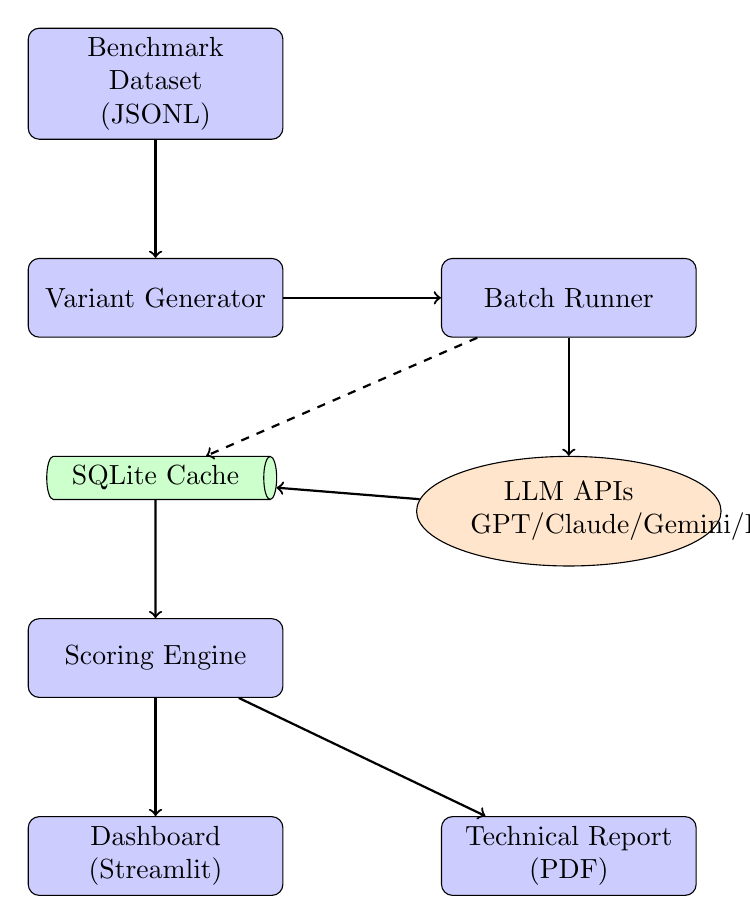
\begin{tikzpicture}[
    node distance=1.5cm,
    box/.style={rectangle, draw, fill=blue!20, text width=3cm, text centered, rounded corners, minimum height=1cm},
    storage/.style={cylinder, draw, fill=green!20, text width=2.5cm, text centered, minimum height=1cm, aspect=0.3},
    cloud/.style={ellipse, draw, fill=orange!20, text width=2.5cm, text centered, minimum height=1cm}
]

% Top Layer - Data Sources
\node[box] (dataset) {Benchmark Dataset\\(JSONL)};

% Middle Layer - Processing
\node[box, below=of dataset] (generator) {Variant Generator};
\node[box, right=2cm of generator] (runner) {Batch Runner};

% Storage
\node[storage, below=of generator] (cache) {SQLite Cache};

% APIs
\node[cloud, below=of runner] (apis) {LLM APIs\\GPT/Claude/Gemini/Llama};

% Evaluation
\node[box, below=of cache] (scorer) {Scoring Engine};

% Output
\node[box, below=of scorer] (dashboard) {Dashboard\\(Streamlit)};
\node[box, right=2cm of dashboard] (report) {Technical Report\\(PDF)};

% Arrows
\draw[->, thick] (dataset) -- (generator);
\draw[->, thick] (generator) -- (runner);
\draw[->, thick] (runner) -- (apis);
\draw[->, thick] (apis) -- (cache);
\draw[->, thick] (cache) -- (scorer);
\draw[->, thick] (scorer) -- (dashboard);
\draw[->, thick] (scorer) -- (report);
\draw[->, thick, dashed] (runner) -- (cache);

\end{tikzpicture}
\caption{System architecture overview}
\end{figure}

\subsection{Component Descriptions}

\begin{enumerate}[leftmargin=*]
    \item \textbf{Benchmark Dataset}: JSONL files containing base prompts, variants, and ground truth
    
    \item \textbf{Variant Generator}: Produces multiple equivalent versions of each prompt using:
    \begin{itemize}
        \item Template-based transformations
        \item LLM-powered paraphrasing
        \item Rule-based formatting changes
    \end{itemize}
    
    \item \textbf{Batch Runner}: Orchestrates parallel execution across multiple models:
    \begin{itemize}
        \item Rate limiting and retry logic
        \item Progress tracking
        \item Error recovery
    \end{itemize}
    
    \item \textbf{SQLite Cache}: Stores responses to avoid duplicate API calls:
    \begin{itemize}
        \item Key: hash(prompt + model + parameters)
        \item Value: response + metadata + timestamp
    \end{itemize}
    
    \item \textbf{LLM APIs}: External model providers (OpenAI, Anthropic, Google, Together)
    
    \item \textbf{Scoring Engine}: Computes metrics:
    \begin{itemize}
        \item Schema validation (JSON tasks)
        \item Embedding similarity
        \item Answer correctness
        \item Aggregate statistics
    \end{itemize}
    
    \item \textbf{Dashboard}: Interactive Streamlit application for exploration
    
    \item \textbf{Technical Report}: LaTeX-generated PDF with findings
\end{enumerate}

\section{Detailed Flowcharts}

\subsection{Overall System Workflow}

\begin{figure}[h]
\centering
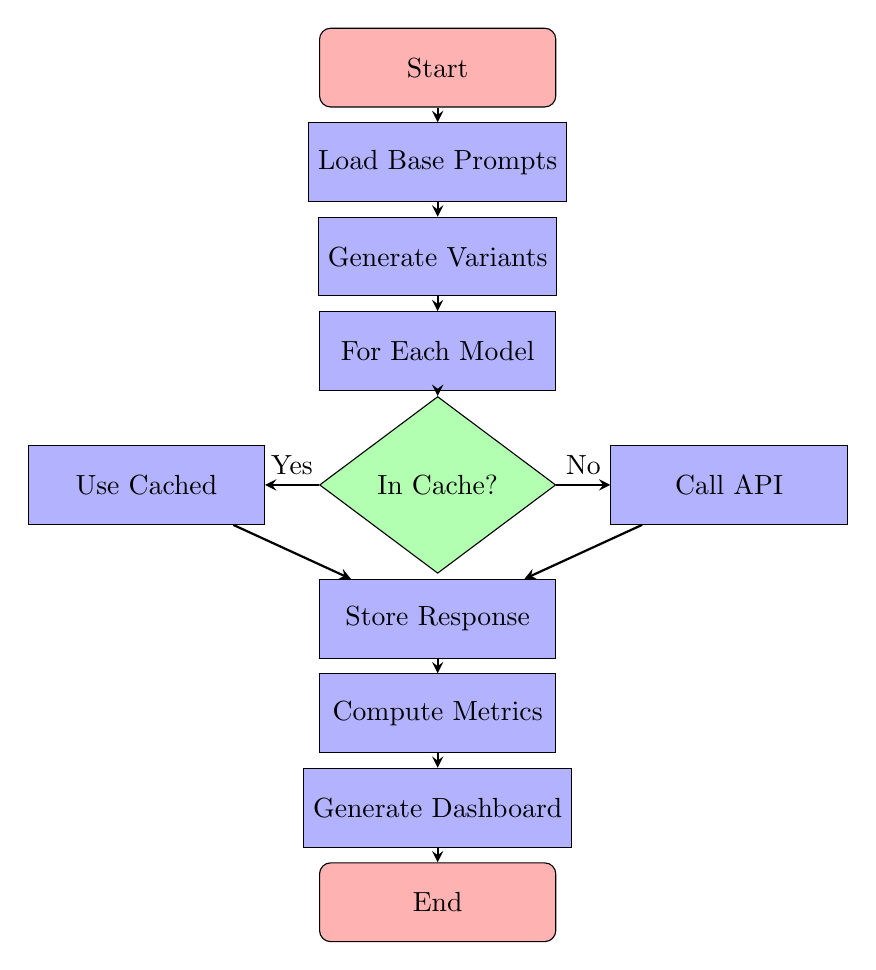
\begin{tikzpicture}[node distance=1.2cm]
\tikzstyle{startstop} = [rectangle, rounded corners, minimum width=3cm, minimum height=1cm,text centered, draw=black, fill=red!30]
\tikzstyle{process} = [rectangle, minimum width=3cm, minimum height=1cm, text centered, draw=black, fill=blue!30]
\tikzstyle{decision} = [diamond, minimum width=3cm, minimum height=1cm, text centered, draw=black, fill=green!30]
\tikzstyle{arrow} = [thick,->,>=stealth]

\node (start) [startstop] {Start};
\node (loaddata) [process, below of=start] {Load Base Prompts};
\node (genvariants) [process, below of=loaddata] {Generate Variants};
\node (models) [process, below of=genvariants] {For Each Model};
\node (checkcache) [decision, below of=models, yshift=-0.5cm] {In Cache?};
\node (callapi) [process, right of=checkcache, xshift=2.5cm] {Call API};
\node (usecache) [process, left of=checkcache, xshift=-2.5cm] {Use Cached};
\node (store) [process, below of=checkcache, yshift=-0.5cm] {Store Response};
\node (score) [process, below of=store] {Compute Metrics};
\node (viz) [process, below of=score] {Generate Dashboard};
\node (end) [startstop, below of=viz] {End};

\draw [arrow] (start) -- (loaddata);
\draw [arrow] (loaddata) -- (genvariants);
\draw [arrow] (genvariants) -- (models);
\draw [arrow] (models) -- (checkcache);
\draw [arrow] (checkcache) -- node[anchor=south] {No} (callapi);
\draw [arrow] (checkcache) -- node[anchor=south] {Yes} (usecache);
\draw [arrow] (callapi) -- (store);
\draw [arrow] (usecache) -- (store);
\draw [arrow] (store) -- (score);
\draw [arrow] (score) -- (viz);
\draw [arrow] (viz) -- (end);

\end{tikzpicture}
\caption{Main execution workflow}
\end{figure}

\subsection{Variant Generation Process}

\begin{figure}[h]
\centering
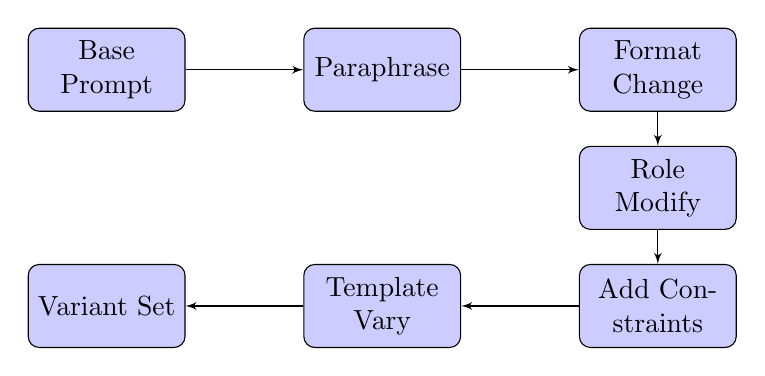
\begin{tikzpicture}[node distance=1.5cm, auto]
\tikzstyle{block} = [rectangle, draw, fill=blue!20, text width=5em, text centered, rounded corners, minimum height=3em]
\tikzstyle{line} = [draw, -latex']

\node [block] (input) {Base Prompt};
\node [block, right of=input, xshift=2cm] (paraphrase) {Paraphrase};
\node [block, right of=paraphrase, xshift=2cm] (format) {Format Change};
\node [block, below of=format] (role) {Role Modify};
\node [block, below of=role] (constraint) {Add Constraints};
\node [block, left of=constraint, xshift=-2cm] (template) {Template Vary};
\node [block, left of=template, xshift=-2cm] (output) {Variant Set};

\path [line] (input) -- (paraphrase);
\path [line] (paraphrase) -- (format);
\path [line] (format) -- (role);
\path [line] (role) -- (constraint);
\path [line] (constraint) -- (template);
\path [line] (template) -- (output);

\end{tikzpicture}
\caption{Variant generation pipeline}
\end{figure}

\section{Dataset Specification}

\subsection{Task 1: JSON Extraction}

\subsubsection{Example Schema - E-commerce Product}

\begin{lstlisting}[language=json, caption=Product extraction schema]
{
  "type": "object",
  "required": ["product_name", "price", "category"],
  "properties": {
    "product_name": {"type": "string"},
    "price": {"type": "number", "minimum": 0},
    "category": {"type": "string"},
    "brand": {"type": "string"},
    "in_stock": {"type": "boolean"},
    "rating": {"type": "number", "minimum": 0, "maximum": 5}
  }
}
\end{lstlisting}

\subsubsection{Sample Input Document}

\begin{lstlisting}[caption=Example product description]
The Sony WH-1000XM5 wireless headphones are premium 
noise-cancelling headphones priced at $399.99. They fall 
under the Electronics category and are manufactured by Sony. 
Currently in stock with a customer rating of 4.7 out of 5 
stars based on 2,341 reviews.
\end{lstlisting}

\subsubsection{Ground Truth Output}

\begin{lstlisting}[language=json, caption=Expected JSON extraction]
{
  "product_name": "Sony WH-1000XM5",
  "price": 399.99,
  "category": "Electronics",
  "brand": "Sony",
  "in_stock": true,
  "rating": 4.7
}
\end{lstlisting}

\subsubsection{Prompt Variants (Examples)}

\textbf{Variant 1 - Direct}:
\begin{quote}
\textit{Extract the product information from the text into JSON format following the schema.}
\end{quote}

\textbf{Variant 2 - Paraphrased}:
\begin{quote}
\textit{Please parse the following product description and return structured data matching the provided JSON schema.}
\end{quote}

\textbf{Variant 3 - Role-based}:
\begin{quote}
\textit{You are a data extraction specialist. Your task is to convert unstructured product descriptions into structured JSON...}
\end{quote}

\textbf{Variant 4 - Few-shot}:
\begin{quote}
\textit{Here are two examples of product extraction:\\ 
Example 1: [input] → [output]\\
Example 2: [input] → [output]\\
Now extract: [new input]}
\end{quote}

\subsection{Task 2: Grounded Question Answering}

\subsubsection{Sample Context Paragraph}

\begin{quote}
\textit{The Python programming language was created by Guido van Rossum and first released in 1991. Python emphasizes code readability with its notable use of significant indentation. Its language constructs aim to help programmers write clear, logical code for small and large-scale projects. Python is dynamically typed and garbage-collected.}
\end{quote}

\subsubsection{Sample Question}

\textbf{Question}: When was Python first released and who created it?

\subsubsection{Ground Truth Answer}

\begin{quote}
\textit{Python was first released in 1991 and was created by Guido van Rossum.}

\textbf{Supporting Quote}: "The Python programming language was created by Guido van Rossum and first released in 1991."
\end{quote}

\subsubsection{Evaluation Criteria}

\begin{itemize}[leftmargin=*]
    \item Answer must be factually correct
    \item Answer must be grounded in provided context (no hallucination)
    \item Ideally includes citation or quote from context
    \item Should not add information beyond the context
\end{itemize}

\subsection{Dataset Statistics}

\begin{table}[h]
\centering
\begin{tabular}{@{}lrrr@{}}
\toprule
\textbf{Category} & \textbf{Base Prompts} & \textbf{Variants Each} & \textbf{Total} \\ \midrule
JSON Extraction & 50 & 20 & 1,000 \\
Grounded Q\&A & 50 & 20 & 1,000 \\
\textbf{Total} & \textbf{100} & \textbf{—} & \textbf{2,000} \\ \bottomrule
\end{tabular}
\caption{Dataset composition}
\end{table}

\begin{table}[h]
\centering
\begin{tabular}{@{}lr@{}}
\toprule
\textbf{Variant Type} & \textbf{Count per Base} \\ \midrule
Paraphrases & 5 \\
Format changes & 4 \\
Role modifications & 3 \\
Constraint additions & 3 \\
Template variations & 5 \\
\textbf{Total} & \textbf{20} \\ \bottomrule
\end{tabular}
\caption{Variant distribution}
\end{table}

\section{Model Comparison and Analysis}

\subsection{Model Selection Rationale}

\begin{table}[h]
\centering
\small
\begin{tabular}{@{}p{3cm}p{3cm}p{3cm}p{3cm}@{}}
\toprule
\textbf{Model} & \textbf{Provider} & \textbf{Strengths} & \textbf{Cost/1M tokens} \\ \midrule
GPT-4-turbo & OpenAI & Instruction following, JSON mode & \$10 input / \$30 output \\
Claude 3.5 Sonnet & Anthropic & Reasoning, long context & \$3 input / \$15 output \\
Gemini 1.5 Pro & Google & Multimodal ready, fast & \$1.25 input / \$5 output \\
Llama 3.1 70B & Meta (Together) & Open source, cost-effective & \$0.88 input / \$0.88 output \\ \bottomrule
\end{tabular}
\caption{Model comparison}
\end{table}

\subsection{Expected Performance Hypotheses}

\begin{enumerate}[leftmargin=*]
    \item \textbf{JSON Extraction Task}:
    \begin{itemize}
        \item GPT-4 expected to have highest format compliance (JSON mode)
        \item Claude may have better semantic understanding
        \item Llama may struggle with complex schemas
    \end{itemize}
    
    \item \textbf{Grounded Q\&A Task}:
    \begin{itemize}
        \item Claude expected to excel at citation and reasoning
        \item GPT-4 may have more hallucination resistance
        \item Gemini performance unknown (newer model)
    \end{itemize}
    
    \item \textbf{Robustness}:
    \begin{itemize}
        \item Larger models (GPT-4, Claude) expected more stable
        \item Open-source models may show higher variance
        \item Role-based prompts may help smaller models
    \end{itemize}
\end{enumerate}

\subsection{Evaluation Metrics Details}

\subsubsection{Robustness Score}

\[
\text{Robustness} = 1 - \frac{\sigma_{\text{variants}}}{\mu_{\text{accuracy}}}
\]

Where:
\begin{itemize}
    \item $\sigma_{\text{variants}}$ = standard deviation of accuracy across variants
    \item $\mu_{\text{accuracy}}$ = mean accuracy
    \item Higher score = more consistent behavior
\end{itemize}

\subsubsection{Semantic Consistency}

\[
\text{Consistency} = \frac{1}{n(n-1)} \sum_{i \neq j} \text{cosine}(\mathbf{e}_i, \mathbf{e}_j)
\]

Where:
\begin{itemize}
    \item $\mathbf{e}_i$ = embedding of output from variant $i$
    \item $n$ = number of variants
    \item Range: [0, 1], higher = more consistent
\end{itemize}

\subsubsection{Format Compliance Rate}

\[
\text{Compliance} = \frac{\text{Outputs passing schema validation}}{\text{Total outputs}}
\]

\section{Project Timeline (Gantt Chart)}

\begin{figure}[h]
\centering
\begin{ganttchart}[
    hgrid,
    vgrid,
    x unit=0.5cm,
    y unit title=0.7cm,
    y unit chart=0.6cm,
    title height=1,
    bar/.append style={fill=blue!50},
    bar height=0.6
]{1}{28}
\gantttitle{Project Timeline (4 Weeks)}{28} \\
\gantttitle{Week 1}{7}
\gantttitle{Week 2}{7}
\gantttitle{Week 3}{7}
\gantttitle{Week 4}{7} \\

\ganttbar{Schema Design}{1}{3} \\
\ganttbar{Q\&A Dataset}{2}{4} \\
\ganttbar{Variant Generator}{3}{5} \\
\ganttbar{Generate Variants}{5}{7} \\

\ganttbar{API Integration}{8}{10} \\
\ganttbar{Batch Engine}{9}{11} \\
\ganttbar{Metrics Implementation}{11}{13} \\
\ganttbar{Baseline Run}{13}{14} \\

\ganttbar{Full Execution}{15}{17} \\
\ganttbar{Adversarial Tests}{16}{18} \\
\ganttbar{Parameter Study}{18}{20} \\
\ganttbar{Analysis}{19}{21} \\

\ganttbar{Dashboard}{22}{24} \\
\ganttbar{Report Writing}{23}{26} \\
\ganttbar{Presentation Prep}{25}{27} \\
\ganttbar{Final Review}{27}{28}

\end{ganttchart}
\caption{Detailed project Gantt chart}
\end{figure}

\subsection{Daily Task Breakdown - Week 1}

\begin{table}[h]
\centering
\small
\begin{tabular}{@{}lp{10cm}@{}}
\toprule
\textbf{Day} & \textbf{Tasks} \\ \midrule
Mon Feb 24 & Project setup, repo creation, environment config \\
Tue Feb 25 & Design 5 JSON schemas, create sample documents \\
Wed Feb 26 & Label ground truth for JSON task (Milestone 1) \\
Thu Feb 27 & Create Q\&A context paragraphs, write questions \\
Fri Feb 28 & Implement variant generator core logic \\
Sat Mar 1 & Test generator, review quality \\
Sun Mar 2 & Generate all variants, validate dataset (Milestone 2) \\ \bottomrule
\end{tabular}
\caption{Week 1 daily tasks}
\end{table}

\section{Presentation Materials}

\subsection{7-Slide Deck Outline}

\begin{enumerate}[leftmargin=*]
    \item \textbf{Slide 1 - Title}
    \begin{itemize}
        \item Project name: Prompt Crash-Test Lab
        \item Subtitle: LLM Robustness Benchmark
        \item Team members
    \end{itemize}
    
    \item \textbf{Slide 2 - Problem \& Motivation}
    \begin{itemize}
        \item LLMs are inconsistent (20-40\% variance)
        \item No standard testing framework
        \item Real-world risks: broken systems, cost overruns
    \end{itemize}
    
    \item \textbf{Slide 3 - Objectives}
    \begin{itemize}
        \item Create benchmark dataset (2000 variants)
        \item Test 4 models systematically
        \item Quantify robustness with metrics
        \item Identify best practices
    \end{itemize}
    
    \item \textbf{Slide 4 - Approach}
    \begin{itemize}
        \item Two tasks: JSON + Q\&A
        \item Automated variant generation
        \item Multi-model evaluation
        \item Comprehensive metrics
    \end{itemize}
    
    \item \textbf{Slide 5 - Technical Architecture}
    \begin{itemize}
        \item System diagram (use Figure from Appendix)
        \item Key components
        \item Tech stack
    \end{itemize}
    
    \item \textbf{Slide 6 - Expected Results}
    \begin{itemize}
        \item Robustness leaderboard
        \item Interactive dashboard mockup
        \item Sample findings
    \end{itemize}
    
    \item \textbf{Slide 7 - Deliverables \& Timeline}
    \begin{itemize}
        \item Dataset (open-source)
        \item Framework + Dashboard
        \item Technical report
        \item 4-week timeline
    \end{itemize}
\end{enumerate}

\subsection{Q\&A Preparation}

\subsubsection{Likely Questions and Answers}

\textbf{Q1: How do you ensure semantic equivalence of variants?}

\textit{A: We use a combination of LLM-powered paraphrasing with manual validation of a 10\% sample. We also measure semantic similarity using embeddings and only keep variants above 0.85 cosine similarity to the base prompt.}

\vspace{0.3cm}

\textbf{Q2: What if API costs exceed budget?}

\textit{A: We have aggressive caching (SQLite) to avoid duplicate calls. We'll also test on a subset first (20 prompts) to estimate costs. If needed, we can reduce dataset size or use fewer model parameters.}

\vspace{0.3cm}

\textbf{Q3: Why only 2 tasks instead of more?}

\textit{A: We want depth over breadth. Two well-chosen tasks (structured + unstructured) allow thorough analysis within our timeline. Future work can extend to more task types.}

\vspace{0.3cm}

\textbf{Q4: How is this different from existing benchmarks like HELM?}

\textit{A: HELM focuses on absolute performance across tasks. We focus specifically on prompt robustness—testing if the same task with different phrasing yields consistent results. This is critical for real-world deployment but underexplored.}

\vspace{0.3cm}

\textbf{Q5: Can your framework be used by others?}

\textit{A: Yes! We're open-sourcing everything: dataset, code, and methodology. Others can run our benchmark or add new tasks/models. Reproducibility is a core goal.}

\section{References and Citations}

\begin{enumerate}[leftmargin=*]
    \item Brown, T. et al. (2020). "Language Models are Few-Shot Learners." \textit{NeurIPS}. \\
    \textit{Context: GPT-3 architecture, few-shot learning capabilities}
    
    \item Zhao, Z. et al. (2021). "Calibrate Before Use: Improving Few-Shot Performance of Language Models." \textit{ICML}. \\
    \textit{Context: Prompt sensitivity and calibration techniques}
    
    \item Wei, J. et al. (2022). "Chain-of-Thought Prompting Elicits Reasoning in Large Language Models." \textit{NeurIPS}. \\
    \textit{Context: Prompt engineering methodologies}
    
    \item Liang, P. et al. (2022). "Holistic Evaluation of Language Models (HELM)." \textit{arXiv:2211.09110}. \\
    \textit{Context: Comprehensive LLM benchmarking framework}
    
    \item Ouyang, L. et al. (2022). "Training Language Models to Follow Instructions with Human Feedback." \textit{NeurIPS}. \\
    \textit{Context: Instruction following and RLHF}
    
    \item Perez, E. et al. (2022). "Red Teaming Language Models with Language Models." \textit{EMNLP}. \\
    \textit{Context: Adversarial testing of LLMs}
    
    \item Reimers, N. \& Gurevych, I. (2019). "Sentence-BERT: Sentence Embeddings using Siamese BERT-Networks." \textit{EMNLP}. \\
    \textit{Context: Embedding-based similarity measurement}
    
    \item OpenAI (2023). "GPT-4 Technical Report." \textit{arXiv:2303.08774}. \\
    \textit{Context: GPT-4 capabilities and limitations}
    
    \item Anthropic (2024). "Claude 3 Model Card." \\
    \textit{Context: Claude 3.5 Sonnet specifications}
    
    \item Touvron, H. et al. (2023). "Llama 2: Open Foundation and Fine-Tuned Chat Models." \textit{arXiv:2307.09288}. \\
    \textit{Context: Llama model architecture and training}
\end{enumerate}

\section{Appendix: Code Examples}

\subsection{Sample Variant Generator}

\begin{lstlisting}[language=Python, caption=Variant generator pseudocode]
def generate_variants(base_prompt: str, num_variants: int = 20):
    variants = []
    
    # Paraphrasing (5 variants)
    for i in range(5):
        paraphrased = llm_paraphrase(base_prompt, temperature=0.7)
        variants.append({"type": "paraphrase", "text": paraphrased})
    
    # Format changes (4 variants)
    formats = ["markdown", "plaintext", "numbered", "bulleted"]
    for fmt in formats:
        formatted = apply_format(base_prompt, fmt)
        variants.append({"type": "format", "text": formatted})
    
    # Role modifications (3 variants)
    roles = ["expert", "assistant", "teacher"]
    for role in roles:
        modified = f"You are a {role}. {base_prompt}"
        variants.append({"type": "role", "text": modified})
    
    # Constraints (3 variants)
    constraints = [
        "Be concise. " + base_prompt,
        "Provide detailed explanation. " + base_prompt,
        "Use simple language. " + base_prompt
    ]
    variants.extend([{"type": "constraint", "text": c} 
                     for c in constraints])
    
    # Templates (5 variants)
    templates = generate_few_shot_templates(base_prompt)
    variants.extend([{"type": "template", "text": t} 
                     for t in templates])
    
    return variants
\end{lstlisting}

\subsection{Sample Scoring Function}

\begin{lstlisting}[language=Python, caption=Robustness scoring]
def compute_robustness(outputs: List[dict], ground_truth: dict):
    # JSON schema validation
    valid_count = sum(1 for o in outputs 
                     if validate_schema(o["response"]))
    compliance = valid_count / len(outputs)
    
    # Semantic consistency
    embeddings = [get_embedding(o["response"]) 
                  for o in outputs]
    similarities = []
    for i, emb1 in enumerate(embeddings):
        for j, emb2 in enumerate(embeddings[i+1:]):
            sim = cosine_similarity(emb1, emb2)
            similarities.append(sim)
    consistency = np.mean(similarities)
    
    # Accuracy
    correct_count = sum(1 for o in outputs 
                       if matches_ground_truth(o["response"], 
                                               ground_truth))
    accuracy = correct_count / len(outputs)
    
    # Robustness = low variance + high accuracy
    robustness = accuracy * (1 - np.std([accuracy]))
    
    return {
        "robustness": robustness,
        "compliance": compliance,
        "consistency": consistency,
        "accuracy": accuracy
    }
\end{lstlisting}

\section{Budget Breakdown}

\begin{table}[h]
\centering
\begin{tabular}{@{}lrrr@{}}
\toprule
\textbf{Item} & \textbf{Quantity} & \textbf{Cost/Unit} & \textbf{Total} \\ \midrule
GPT-4 API calls & 500 prompts & \$0.15 & \$75 \\
Claude API calls & 500 prompts & \$0.08 & \$40 \\
Gemini API calls & 500 prompts & \$0.03 & \$15 \\
Llama API calls & 500 prompts & \$0.02 & \$10 \\
Variant generation (GPT-4) & 100 prompts & \$0.30 & \$30 \\
Embedding API & 2000 texts & \$0.01 & \$20 \\
Buffer (15\%) & — & — & \$29 \\
\midrule
\textbf{Total Estimated Cost} & & & \textbf{\$219} \\ 
\textbf{Target Budget} & & & \textbf{\$200} \\
\textbf{Optimization Needed} & & & \textbf{-\$19} \\ \bottomrule
\end{tabular}
\caption{API cost estimation}
\end{table}

\textbf{Cost reduction strategies:}
\begin{itemize}
    \item Reduce dataset to 90 base prompts (saves \$20)
    \item Use GPT-3.5 for variant generation (saves \$20)
    \item Aggressive caching (50\% hit rate saves \$40)
\end{itemize}

\section{Success Metrics Summary}

\begin{table}[h]
\centering
\begin{tabular}{@{}lp{8cm}@{}}
\toprule
\textbf{Metric} & \textbf{Target} \\ \midrule
Dataset completeness & 100 base prompts, 2000 variants, 100\% labeled \\
Framework functionality & All 4 models integrated, <2\% error rate \\
Execution success & >95\% of prompts successfully evaluated \\
Statistical significance & p < 0.05 for model comparisons \\
Budget adherence & ≤ \$200 API costs \\
Code quality & >70\% test coverage, documented \\
Deliverable completeness & Dataset + Framework + Dashboard + Report \\
Presentation readiness & 7-minute deck + demo + Q\&A prep \\ \bottomrule
\end{tabular}
\caption{Project success criteria}
\end{table}

\newpage

\section{Conclusion}

This project addresses a critical gap in LLM deployment practices by creating the first comprehensive benchmark specifically focused on \textbf{prompt robustness}. While existing benchmarks like HELM measure absolute performance, our framework quantifies consistency—a crucial factor for production systems where minor prompt variations shouldn't cause dramatic behavioral changes.

Our systematic approach combines automated variant generation, multi-model evaluation, and rigorous statistical analysis to produce actionable insights for practitioners. The deliverables (open-source dataset, evaluation framework, and dashboard) will enable both researchers and engineers to make evidence-based decisions about prompt design and model selection.

Within the 4-week timeline and \$200 budget, this project demonstrates feasibility while maintaining research rigor. The methodologies developed here can be extended to additional tasks, models, and languages in future work.

\vspace{1cm}

\begin{center}
\textbf{For questions or collaboration opportunities:}\\
\vspace{0.3cm}
\texttt{your.email@university.edu}\\
\vspace{0.2cm}
GitHub: \texttt{https://github.com/yourusername/prompt-crashtest-lab}
\end{center}

\end{document}
